\documentclass[10pt]{article}

\usepackage{AMIA}
\usepackage{lipsum}

\usepackage{graphicx}


\title{Title of Your Submission}
\author[1]{Firstname A. Lastname, Degrees}
\author[2]{Firstname B. Lastname, Degrees}
% \author[1,2]{Author Three, PhD}
\affil[1]{Institution City, State, Country (if applicable)}
\affil[2]{Institution City, State, Country (if applicable)}

\begin{document}

\maketitle

\section*{Abstract}
\textit{125-150 words \\ \lipsum[1]}

\section*{Introduction}
\lipsum[3-8]
\cite{he2016deep}

\begin{figure}
    \centering
    \setlength{\abovecaptionskip}{0pt}
    % \includegraphics[width=0.9\textwidth, trim=1.7cm 7cm 8.5cm 2cm, clip]{img/figure1.pdf} % Could crop PDF
    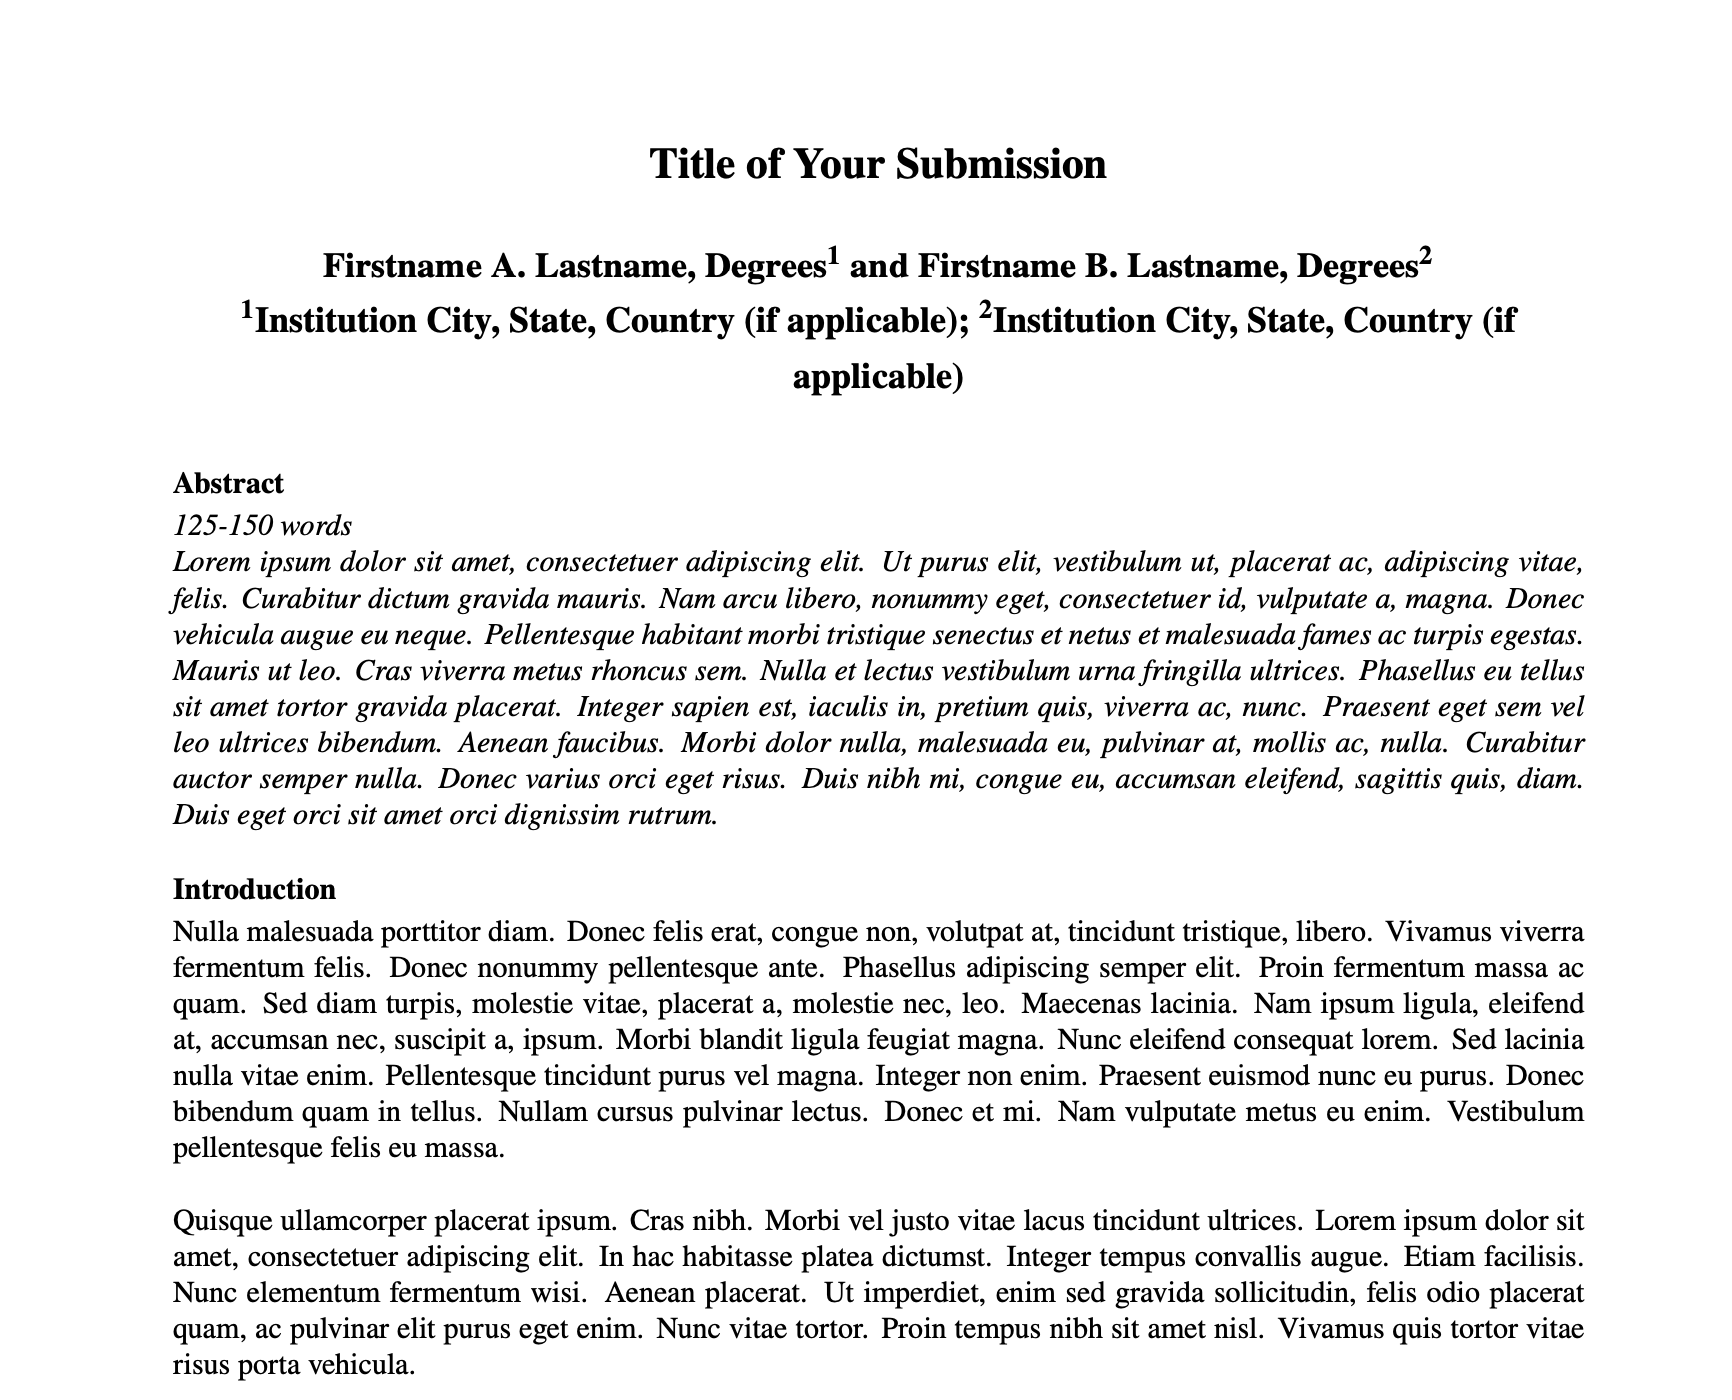
\includegraphics[width=0.4\textwidth]{img/example.png}
    \caption{This is a image.}
    \label{fig::img}
\end{figure}

\begin{table}[hbt!]
\setlength{\abovecaptionskip}{5pt}
\caption{This is Table 2.}
\centering
\resizebox{13cm}{!}{
\begin{tabular}{cccccc}
    \toprule
    \textbf{Table} & \textbf{Table} & \textbf{Within 6 Table} & \textbf{Within 12 Table} & \textbf{Within 24 Table} & \textbf{No Table} \\ 
    \midrule
    \multirow{4}{*}{\textbf{Big Table}}   
        & Table &  &  &  &  \\
        & Table &  &  &  &  \\
        & Table &  &  &  &  \\
        & Table &  &  &  &  \\
    \cline{1-6}
\end{tabular}
}
\label{tab::reuslt}
\end{table}

% References
\bibliographystyle{vancouver}
\bibliography{citation}

\end{document}
